\section{Sizing details} \label{sec:sizeinputs}

The following simplified sizing may be used to give the input sizes for a
cost model.
The storage sizes are given in \tabref{tab:storageFloorOps}
while the compute is given in \tabref{tab:drpAndAlertSizing}
and \tabref{tab:lspSizing}. The cumulative storage requirements are also shown
in \figref{fig:storage}. The cumulative processing required is shown below
in \figref{fig:cores}.

\begin{figure}
\begin{center}
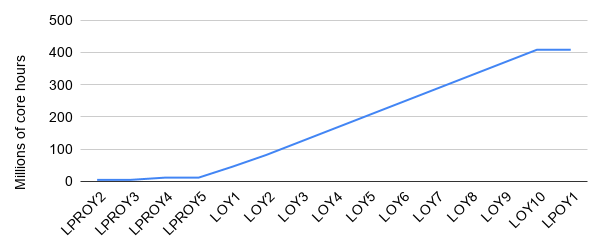
\includegraphics[width=0.8\textwidth]{figs/cores}
\end{center}
\caption{Evolution of {\bf cumulative} computing needs for Rubin Observatory. Details are given below. Compute at other data facilities, is not included here. The \gls{USDF} is responsible for the last two years of pre operations (LPROY4-5) which are transition to \gls{USDF}, the survey years (LOY1-10), and the post operations years (only the first year of two is shown).\label{fig:cores}}
\end{figure}

Some useful inputs are provided in \tabref{tab:Inputs}.

\tiny \begin{longtable} { |p{0.22\textwidth}  |r  |r  |r  |r  |r  |r |} 
\caption{Various inputs for deriving costs - 2019 represents current holdings. \label{tab:Inputs}}\\ 
\hline 
\textbf{Year}&\textbf{2019}&\textbf{2020}&\textbf{2021}&\textbf{2022}&\textbf{2023} \\ \hline
{Core-hours Needed Total (DRP)}&{}&{4.41E+06}&{4.41E+06}&{1.12E+07}&{4.53E+07} \\ \hline
{Annual Increase}&{}&{4.41E+06}&{0.00E+00}&{6.81E+06}&{3.40E+07} \\ \hline
{Time to Process days}&{}&{100.0}&{100.0}&{100.0}&{200} \\ \hline
{Time to Process hours}&{}&{2,400}&{2,400}&{2,400}&{4,800} \\ \hline
{Instantaneous cores (DRP) Total}&{}&{1,836}&{1,836}&{4,673}&{9,430} \\ \hline
{Instantaneous cores (DRP) Annual increase}&{1152}&{1,836}&{0}&{2,837}&{7,093} \\ \hline
{Instantaneous cores (Alerts)}&{}&{0}&{0}&{1188}&{1188} \\ \hline
{Cores (Alerts) Annual increase}&{}&{0}&{0}&{1188}&{0} \\ \hline
{Instantaneous cores (US DAC/ Staff)}&{540}&{540}&{540}&{141}&{568} \\ \hline
{Cores (US DAC/ Staff) Annual increase}&{}&{0}&{0}&{0}&{428} \\ \hline
{Instantaneous cores (Chilean DAC)}&{}&{0}&{0}&{26}&{103} \\ \hline
{Cores (Chilean DAC) Annual increase}&{}&{0}&{0}&{26}&{78} \\ \hline
{Qserv nodes (US DAC/ Staff)}&{}&{}&{}&{14}&{95} \\ \hline
{Qserv nodes (US DAC/ Staff) Annual Increase}&{}&{}&{}&{14}&{81} \\ \hline
{Qserv nodes (Chilean DAC)}&{}&{}&{}&{14}&{95} \\ \hline
{Qserv nodes (Chilean DAC) Annual Increase}&{}&{}&{}&{14}&{81} \\ \hline
\textbf{Total Cores Annual Increase}&\textbf{}&\textbf{1,836}&\textbf{0}&\textbf{4,051}&\textbf{7,599} \\ \hline
{Fast Storage (TB)}&{}&{12}&{24}&{50}&{206} \\ \hline
{Annual Increase (Fast)}&{}&{12}&{12}&{26}&{156} \\ \hline
{Normal Storage (TB)}&{3000}&{3680}&{3748}&{9241}&{38983} \\ \hline
{Annual Increase (Normal)}&{}&{680}&{68}&{5494}&{29742} \\ \hline
{Latent Storage  (TB)}&{}&{319}&{876}&{4966}&{28854} \\ \hline
{Annual Increase (Latent)}&{}&{319}&{557}&{4090}&{23888} \\ \hline
{High Latency (TB)}&{}&{2910}&{6128}&{16733}&{63245} \\ \hline
{Annual Increase (High Latency)}&{}&{2910}&{3218}&{10605}&{46512} \\ \hline
{Chilean DAC Fast Storage (TB)}&{}&{}&{}&{}&{156} \\ \hline
{Annual Increase (Fast Chilean DAC)}&{}&{}&{}&{}&{156} \\ \hline
{Chilean DAC Latent Storage (TB)}&{}&{}&{}&{}&{28854} \\ \hline
{Annual Increase (Latent Chilean DAC)}&{}&{}&{}&{}&{28854} \\ \hline
{Annual price decrease CPU}&{}&{10\%}&{}&{}&{} \\ \hline
{Annual price decrease Storage}&{}&{5\%}&{}&{}&{} \\ \hline
{Annual price decrease Qserv}&{}&{8\%}&{}&{}&{} \\ \hline
\end{longtable} \normalsize


\subsection{Processing Plan}

This model assumes the following processing:
\begin{itemize}
\item Precursor data (HSC RC2 and a similarly-sized DESC DC2 subset) is reprocessed each month during the Construction period using the Data Release Production (DRP).
\item A large precursor reprocessing of HSC PDR2 (or equivalent) is completed twice a year.
Products from one of these reprocessings will be released as Data Preview 0 (DP0) by the operations team. This will not be done at the \gls{USDF}.
\item One or more of these processings will be devoted to ComCam and LSSTCam science data during Commissioning. Some processing at the \gls{USDF} might occur in the
transition in late FY22. If not then, certainly in FY23 in advance of full operations. ComCam data will be released as DP1. LSSTCam commissioning data will be released as DP2 soon {\it after} the start of full operations in FY24.
\item Alert Production (AP) processing happens continuously as LSSTCam science images are obtained.
AP hardware is purchased in FY23 to support this.
\item DR1 processing begins after the first 6~months of the survey; the hardware for this can be part of the purchase during FY23.
\item Annual DRP execution starts at the beginning of LSST Operations Year 2 with the processing for DR2.
The hardware for each year's processing must be purchased and ready for use at the beginning of the year, so it is allocated in the tables to the prior fiscal year, when the images for that processing were taken.

\end{itemize}

Some storage for raw data needs to be in place at the beginning of the fiscal
year, but it can be ramped up over the course of the year.
As a simplification it is allocated to the fiscal year in which it will be used.

\subsection{Operations Storage Model}

\subsubsection{Overview}

Values are computed for the amount of storage expected to be "on the floor" at the beginning of each fiscal.
Key scientific and algorithmic assumptions made include:
\begin{itemize}
\item All significant intermediates and data products generated by Data Release Production processing need to be kept on filesystem disk until the DRP is complete.
Some scratch space is provided to hold small, temporary intermediates.
If some intermediates could be removed during DRP when it is known they will no longer be needed, some space savings could be realized.
\item HSC RC2 processing is representative of the outputs that DRP will generate (see e.g. PDR2\footnote{https://hsc-release.mtk.nao.ac.jp/doc/index.php/sample-page/pdr2/}
The coadd storage is doubled to account for an additional "good-seeing" coadd along with the existing "deep" coadd.
\item Processed visit images (PVIs) and catalogs in Parquet format start on "normal" filesystem disk but then move to object storage at the completion of the DRP, with lossy compression of the PVIs at that time.
This is in accordance with \jira{RFC-325}, although the relevant LCR has not yet been approved.
Object storage is expected to be cheaper and more scalable for read-only data products; filesystem storage is used for data that is being generated or modified.
\item Raw images and coadd images are only temporarily stored on filesystem disk and are then rapidly moved to object storage, where they are retained.
\item Intermediates like warped images for coaddition are not survey data products and do not need to be kept beyond the end of the DRP and subsequent QA.
\end{itemize}

All data is backed up to tape permanently, including annual snapshots of filesystems.
Any incremental backups are assumed to be reusable or otherwise purged and hence not significant.

\subsubsection{Parameters}

The numbers of science users are estimates, using "Stack Club" users and Commissioning users for FY20 and 2021, followed by US science users in FY22 and FY23 for Data Preview data.
The bulk of US science users are not expected to arrive until after Data Release~1 at the beginning of LOY2.

Storage per science user is estimated based on today's usage at NCSA, scaled up as users become more active, and approaching the number given in \citeds{LSE-81} as Operations begins.
Note that it is expected that there will be a wide distribution of usage by user, with some using almost none and some using much more than their proportional share.

The LSSTCam image size is uncompressed and includes overscan, 4~bytes of raw data per pixel, and both science and corner rafts (guide and focus sensors).

The raw image compression factor was measured on simulated LSST images.
The lossy image compression factor for processed visit images is the ratio between the lossy-compressed file size (estimated at 1/6 of uncompressed) and the lossless-compressed file size (estimated at 66\% of uncompressed).
Note that PVIs do not compress losslessly as well as raw images due to their floating point planes.

The number of observing nights per year and the number of visits per night are maximal estimates.
Two~images per visit is still the baseline and a possibility that must be accounted for.
The number of calibration images per day was derived from the calibration plan.

Two complete all-sky coadds are assumed, one for "good seeing" and one deep.

As stated above, the number of LSSTCam science images is scaled by 2/12 for FY23
given the length of science validation time.
The number of test images, taken on test stands, is estimated as a ramp
up to the full science cadence.
The numbers of engineering (unprocessed) and calibration images are
estimated as ramping-down fractions of the number of science and test images,
with calibration images ending at the number per day given previously.

Sizes of rows in various data product tables are taken from \citeds{LDM-141}, which was in turn derived from the \gls{DPDD}.

Qserv replicates its data for fault tolerance; a typical replication factor is selected here.

\subsubsection{Data Product Sizing}

Images and the results of processing them are the dominant factor controlling the storage sizing which is outlined in \tabref{tab:datasetSizingOps}.
Precursor survey and LSSTCam images are the largest; ComCam, at less than 5\% of the size of LSSTCam and with little on-sky science time is negligible, as is LATISS, which is less than 1\% of the size of LSSTCam, though it has considerable on-sky time.

The sizing of the Alert Production Database (APDB) is based on experiments in \cite{DMTN-113} which found that 57,000 visits took 4.5~TB including indexes.
A simple linear scaling to a full year's visits was performed, with half that purchased in 2020 for large (but not full) scale testing.

HyperSuprime-Cam (HSC) RC2 is a relatively small dataset used for monthly processing tests, but it is highly representative of the currently-known DRP work and so is used as the basis for scaling.
The size of the input images was taken from \cite{DMTN-091}; the size of the outputs (image and Parquet/other non-image files) was measured from the latest execution.
A similar size dataset based on DESC DC2 is assumed to be being used for an additional monthly processing test.
Note that this is a very small subset of the full DESC DC2, which is expected to cover 300~square degrees to 10-year LSST depth (approximately 1000 epochs per point on the sky).
The full DESC DC2 is not currently scheduled to be reprocessed by the construction team.
Instead, twice-a-year processings of the full HSC SSP PDR2 dataset (including PDR1) are assumed to occur.
The size of this dataset was measured on disk; it is 2,564,358 CCD images, each at 18.2~MB (approximately three times the size of PDR1 alone). The Operations
team plans to host DESC DC2 as part of DP0 and may do some reprocessing of
DESC DC2 for training and readiness purposes. But this will not be done at
the \gls{USDF}.

Output sizes are assumed to scale linearly with input size, and by the same factor for each instrument, except for coadds which scale by the sky area processed.
While the Object catalog ought to be proportional to sky area as well, its size is expected to be dominated by Source and ForcedSource, so we conservatively make them all proportional to input size (visits) for the precursor data where we do not have object count estimates.
For LSSTCam, we use the catalog row estimates to derive Qserv table sizes, but the Parquet file sizes are scaled based on HSC, as they may differ from the Qserv schema.

Scratch space is set at 10\% of the output image storage for LSSTCam processing; it is assumed to be already present for precursor processing.

Qserv Czar fast (SSD) storage is assumed to be used for the primary Object table; additional space for the so-called "secondary index" mapping object identifiers to spatial chunks is negligible in comparison.

The main Qserv database storage is based on the Parquet file sizing for precursor data and on the estimated numbers of Objects, Sources, and ForcedSources for LSSTCam data.

Note that no space is explicitly reserved for Qserv query result storage.

An additional 20\% disk and tape storage is added to account for all other needs.

\tiny \begin{longtable} { |p{0.22\textwidth}  |r  |r  |r  |r  |r  |r  |r  |r  |r  |r  |r  |r |} 
\caption{Dataset sizes used to calculate storage needs during Operations \label{tab:datasetSizingOps}}\\ 
\hline 
\textbf{Dataset Sizing}&\textbf{unit}&\textbf{LOY1}&\textbf{LOY2}&\textbf{LOY3}&\textbf{LOY4}&\textbf{LOY5}&\textbf{LOY6}&\textbf{LOY7}&\textbf{LOY8}&\textbf{LOY9}&\textbf{LOY10} \\ \hline
{LSSTCam Area}&{deg\^2}&{17000}&{17000}&{17000}&{17000}&{17000}&{17000}&{17000}&{17000}&{17000}&{17000} \\ \hline
{APDB}&{TB}&{24}&{24}&{24}&{24}&{24}&{24}&{24}&{24}&{24}&{24} \\ \hline
{Object store datasets:}&&&&&&&&&&& \\ \hline
{Incremental LSSTCam Raw Images}&{TB}&{4816}&{4816}&{4816}&{4816}&{4816}&{4816}&{4816}&{4816}&{4816}&{4816} \\ \hline
{LSSTCam Output Coadd Images}&{TB}&{7727}&{7727}&{7727}&{7727}&{7727}&{7727}&{7727}&{7727}&{7727}&{7727} \\ \hline
{Normal disk datasets:}&&&&&&&&&&& \\ \hline
{LSSTCam Output Images}&{TB}&{13485}&{26970}&{40456}&{53941}&{67426}&{80911}&{94397}&{107882}&{121367}&{134852} \\ \hline
{LSSTCam Output Parquet}&{TB}&{7973}&{15946}&{23919}&{31893}&{39866}&{47839}&{55812}&{63785}&{71758}&{79731} \\ \hline
{Scratch}&{TB}&{1349}&{2697}&{4046}&{5394}&{6743}&{8091}&{9440}&{10788}&{12137}&{13485} \\ \hline
{Qserv Czar/ Object}&{TB}&{156}&{190}&{215}&{238}&{258}&{279}&{298}&{318}&{335}&{353} \\ \hline
{Qserv Database}&{TB}&{3510}&{5748}&{8018}&{10378}&{12881}&{15475}&{18199}&{21042}&{23965}&{27010} \\ \hline
{Science User Home}&{TB}&{2000}&{3000}&{4200}&{5250}&{6000}&{6750}&{7500}&{8250}&{9000}&{9750} \\ \hline
{Other/ Misc}&{TB}&{8208}&{13424}&{18684}&{23932}&{29148}&{34382}&{39642}&{44926}&{50226}&{55550} \\ \hline
\end{longtable} \normalsize


\subsubsection{Storage Sizing}

Finally, storage is allocated to specific types as shown in \tabref{tab:storageFloorOps}.
Fast storage (SSD) is used for the APDB and Qserv Czar, which accumulates data from year to year until Data Releases are retired.
Normal storage is used for the datasets labeled as such, including output images (initially), output catalogs, and scratch.
Local Qserv storage is used for Qserv catalogs.
It is assumed that precursor data will be removed from Qserv once LSST data is available, but the LSST data accumulates from year to year.

Raw images (lossless-compressed) are written immediately to object storage, as are Parquet-format catalogs.
PVIs are lossy-compressed and placed in object storage.
The complete set of raw images is available, whereas the catalogs from only the last two Data Releases and the one in preparation are kept, and the PVIs from only the last Data Release and the one in preparation are online.

All data products and new raw images for each Data Release are copied to tape, but scratch space and the Qserv-schema catalogs are not.

Note that no replication is assumed in the object store.

\subsection{Compute Model}


\subsubsection{Overview}
This simplified computing model (\tabref{tab:computeSizingOps}) divides computation into three classes: Data Release Production (DRP), Alert Production, and Rubin Science Platform (for Rubin staff internal use).
Calibration Products Production is assumed to be negligible.
The number of cores for Alert Production does not change with time.

Scaling compute needs based on an execution of the nascent DRP pipeline on HSC PDR1 data and nightly executions of the nascent \texttt{ap\_pipe} pipeline on HiTS2015 data is appropriate, but the fact that several steps are still missing from these pipelines must be taken into account.

Elapsed times are measured on existing hardware and converted into core-hours on a nominal CPU (Intel Xeon E5-2680v3 at 2.50~GHz).
For example, if a pipeline running on precursor data took an average of one hour on a 32-core nominal CPU, 32 core-hours would be used as its compute requirement.
This estimation methodology incorporates all I/O, memory bandwidth, cache miss, and other overheads into the core-hour measurement, simplifying calculations.
Note that the nominal CPU does not evolve with time; if future CPUs do more work per core, the actual core-hours may be less than estimated here.

Scaling to other CPUs of the same architecture is based on the ratios of nominal GHz clock rates and core counts.
For different architectures (e.g. Rome), the scaling is based on the ratio of industry-reported achievable FLOPS for the two architectures.

Key scientific and algorithmic assumptions are:
\begin{itemize}
\item DRP compute time is proportional to the input data size (or, equivalently, the number of visits).
While certain tasks are undoubtedly proportional to sky area or number of Objects, overall the pipeline elapsed times are a better fit to the number of visits.
Some of this may be because the Object density increases as the number of visits to the same sky patch increases.
\item HSC PDR1 processing is generally representative of the final DRP, with an allocation for future additional steps as described below.
\item Qserv node counts should remain proportional to the size of data loaded into the database in order to maintain sufficient disk bandwidth and query processing capability, but the proportionality constant changes with time as new generations of system bus with greater bandwidth become available.
\item The US DAC LSP is sized at 10\% of the DRP compute budget in core-hours, readjusted to be spread over an entire year.
The Rubin staff LSP is sized at 10\% of the US DAC.

\end{itemize}

The DAC and staff LSP instances are sized based on the assumed percentages of DRP compute.

The amount of Qserv data that can be handled by a node is assumed to grow with time, doubling every four years (PCI Express has gone from 1.0~GB/sec to 16~GB/sec between 2003 and 2019).
The number of Qserv nodes is calculated by dividing each Data Release's storage by the storage-per-node figure for its year; older nodes are assumed to be retired.

\subsubsection{Parameters}
The key parameters in \tabref{tab:computeSizingOps} are described below.

HSC PDR1 was executed on the NCSA verification cluster, which uses the nominal CPU.
The Alert Production executes on Kubernetes nodes, which are a bit slower; to be conservative, this is neglected.

A 2018  run of DRP on HSC PDR1 data is described at \url{https://confluence.lsstcorp.org/x/WpBiB}.
The input data size is measured; note that the input data files are lossless-compressed.
Most jobs (but not most of the time) could run on relatively small-memory machines with 24~cores and 5~GB RAM per core.
The largest and longest-running jobs, however, required up to 4~times as much memory, using half or a quarter of the cores.
To be conservative, we assume that half the cores were used for the large-memory jobs.
The percentage of DRP core-hours that will need to execute on large-memory nodes is estimated.

Since the HSC PDR1 processing did not include several steps from the Science Pipelines Design document \citedsp{LDM-151} such as image differencing and full multi-epoch characterization, the core-hours used are scaled up to the expected pipeline consumption.
Note that these algorithmic adjustments are multiplicative.

The SQuaSH system reports the execution time of \texttt{ap\_pipe} in seconds per CCD.
A mean was taken over all processed CCDs, and it was assumed that each CCD is processed on a single core.
These CCDs are from DECam, which is half the size of an LSST CCD, so the total time is doubled.
A factor is added to account for additional steps like differential chromatic refraction compensation and false positive detection that are not well-represented in the current pipeline.
Multiplying by the number of LSSTCam science CCDs gives the total number of core-hours per visit.

The amount of Qserv data that can be handled by one node is estimated based on the amount of disk that can be scanned in 12~hours at an aggregate rate of 1~GB per second.
(Since the Qserv data replicas are not all anticipated to be accessed at the same rate, this is a conservative estimate.)

\subsubsection{Data Release Production}

The number of nominal core-hours per TB of input data is multiplied by the precursor (HSC RC2 and DESC DC2 subset for 12~months and HSC PDR2 twice a year) and LSSTCam input data sizes (with lossless compression) to determine the total number of core-hours needed in each year.
This is shown in \tabref{tab:drpAndAlertSizing}.
Approximately one-third of these core-hours need to be provided by small-memory (4-5~GB/core) machines; the other two-thirds need to come from large-memory (8-20~GB/core) machines.

\tiny \begin{longtable} { |p{0.22\textwidth}  |r  |r  |r  |r  |r  |r  |r |} 
\caption{Compute needs for DRP and AP \label{tab:drpAndAlertSizing}}\\ 
\hline 
\textbf{Data Release Production}&\textbf{units}&\textbf{FY20}&\textbf{FY21}&\textbf{FY22}&\textbf{FY23}&\textbf{Notes} \\ \hline
{Precursor input size}&{TB}&{206}&{206}&{206}&{206}& \\ \hline
{LSSTCam visit input size}&{TB}&{}&{}&{319}&{1911}&{raw images /  images/ visit, lossless-compressed} \\ \hline
{Precursor compute}&{core-hours}&{4.4E+06}&{4.4E+06}&{4.4E+06}&{4.4E+06}& \\ \hline
{LSSTCam compute}&{core-hours}&{}&{}&{6.8E+06}&{4.1E+07}& \\ \hline
\textbf{Total DRP compute}&\textbf{core-hours}&\textbf{4.4E+06}&\textbf{4.4E+06}&\textbf{1.1E+07}&\textbf{4.5E+07}& \\ \hline
{Alert Production}&{units}&{FY20}&{FY21}&{FY22}&{FY23}&{Notes} \\ \hline
{AP cores}&{cores}&{}&{}&{1,188}&{1,188}&{minimum necessary to keep up} \\ \hline
\end{longtable} \normalsize


\subsubsection{Alert Production}

The core-hours per visit are divided by the minimum visit length (30~sec plus 1~sec shutter motion plus 2~sec readout) to give the minimum number of cores needed to keep up with image taking.
This is shown in \tabref{tab:drpAndAlertSizing}.
These cores are expected to be provided over multiple "strings" of nodes.
Note that the current AP design is not readily able to take advantage of more than one core per CCD.

\subsubsection{LSST Science Platform}

LSST Science Platform needs for US DAC science users are derived as 10\% of the DRP core-hour requirement and are shown in \tabref{tab:lspSizing}.
The LSP core-hours are assumed to be spread over a year, giving the total number of nominal cores needed in the DAC.
Peak loads are expected to be handled by "borrowing" elastically from the DRP compute pool.

As a reasonableness check, the number of cores per science user is computed, but it must be noted that an oversubscription factor needs to be taken into account since not all users are expected to be simultaneously active.

Similar computations for the Chilean DAC (at 20\% of the US DAC) and the LSST staff LSP (at 10\% of the US DAC) are also in \tabref{tab:lspSizing}.

The number of Qserv nodes needed is computed from the storage devoted to it and the storage per node number.
Note that staff use of Qserv is taken into account by loading the Data Release products into an internal-only Qserv instance and then making that instance part of the DAC at Data Release, so the compute sizing is part of the US DAC.

\tiny \begin{longtable} { |p{0.22\textwidth}  |r  |r  |r  |r  |r  |r  |r |} 
\caption{Compute needs for the Science Platform instances \label{tab:lspSizing}}\\ 
\hline 
\textbf{US DAC}&\textbf{units}&\textbf{FY20}&\textbf{FY21}&\textbf{FY22}&\textbf{FY23}&\textbf{Notes} \\ \hline
{LSP cores}&{cores}&{}&{}&{128}&{517}&{10\% of DRP, over a year} \\ \hline
{Qserv nodes}&{nodes}&{}&{}&{14}&{95}& \\ \hline
{LSP cores/ science user}&{cores/ user}&{}&{}&{0.03}&{0.10}&{includes oversubscription} \\ \hline
{Chilean DAC}&{units}&{FY20}&{FY21}&{FY22}&{FY23}&{Notes} \\ \hline
{LSP cores}&{cores}&{}&{}&{26}&{103}&{20\% of US DAC} \\ \hline
{Qserv nodes}&{nodes}&{}&{}&{14}&{95}& \\ \hline
{Staff LSP}&{units}&{FY20}&{FY21}&{FY22}&{FY23}&{Notes} \\ \hline
{LSP cores}&{cores}&{}&{}&{13}&{52}&{10\% of US DAC} \\ \hline
\end{longtable} \normalsize


